\documentclass[a4paper,11pt]{article}
\usepackage[left=2.5cm, right=2.5cm, top=2cm, bottom=2.5cm]{geometry}
\usepackage{graphicx}
\usepackage{amssymb}
\usepackage{amsmath}
\usepackage{listings}
\usepackage{color} %red, green, blue, yellow, cyan, magenta, black, white
\definecolor{mygreen}{RGB}{28,172,0} % color values Red, Green, Blue
\definecolor{mylilas}{RGB}{170,55,241}

\begin{document}
\title{\LARGE{\textbf{ECEN 220 Lab 1}}}
\author{Niels Clayton \\300437590}
\date{}
\maketitle

\section*{Part 1: Signal Periodicity}
\begin{figure}[h]
\centering
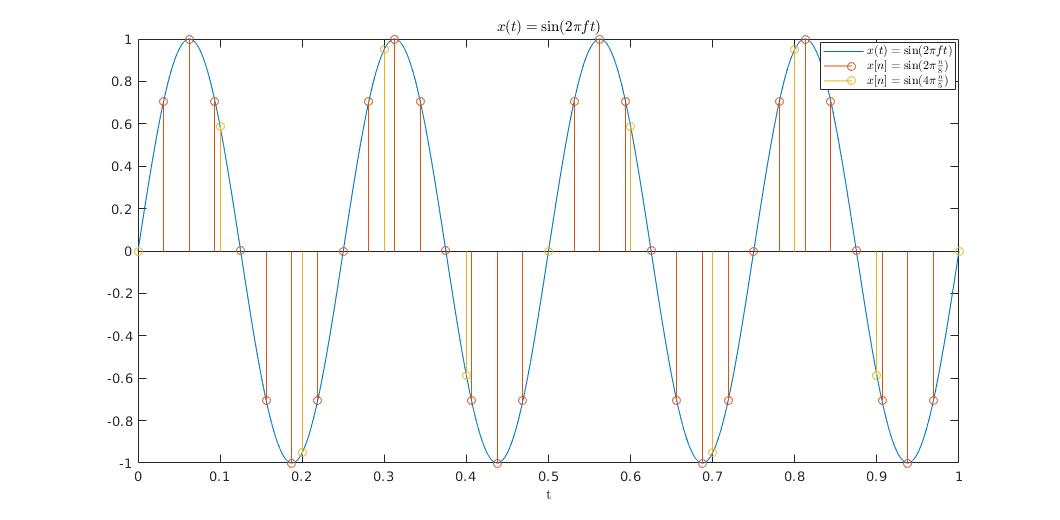
\includegraphics[width=\linewidth]{2.jpg}
\caption{continuous and discrete time plots}
\end{figure}
The period of a continuous time signal can found using $\frac{1}{f_0}=\frac{1}{4}$.\\
The period of a discrete time signal can be found using $\frac{2\pi}{\omega_0} = \frac{N}{M}$, Where N is the period as a number of samples, and M is the number of samples that fit into one cycle of the discrete signal.\\
The period of one sample is one over the sampling frequency.

Using this we can find that:\\ \\
 $x(t)$ has a period of $\frac{1}{4}$ or $0.25s$\\
$x_1[n]$ has a period of 8 samples\\
$x_2[n]$ has a period of 5 samples\\ \\

Using the sampling frequencies of $x_1$ and $x_2$ respectively, we can calculate the time period in terms of seconds. \\ \\
$x_1[n] : 8 \times \frac{1}{32} = 0.25s $ \\
$x_2[n] : 5 \times \frac{1}{10} = 0.5s$ \\ \\

From this we can see that $x_1$ has the same period as $x(t)$, this can be seen in figure 1 above.\\ 
It can also be seen that $x_2$ has a period twice that of $x(t)$, meaning that it repeats ever 2 periods of $x(t)$
\newpage

\section*{Part 2: Linearity}
If a system $f(x)$ is linear, The following rule will be true:\\
$$f(x_1+x_2) = f(x_1)+f(x_2)$$\\ \\
When this test was applied to the system $y[n]=2^{x[n]}$ the two different outputs were plotted against each other in figure 2.\\
Since the two discrete time plots do not match all values, it can be concluded that the system $y[n]=2^{x[n]}$ is not linear.\\ \\
\begin{figure}[h]
\centering
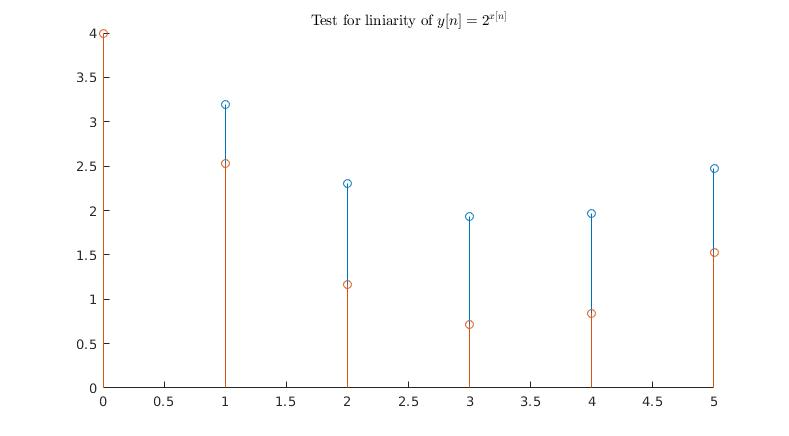
\includegraphics[width=10cm]{linarity_test_1.jpg}
\caption{$f(x_1+x_2) = f(x_1)+f(x_2)$}
\end{figure}

When this test was applied to the system $y[n]=nx[n]$ the two different outputs were plotted against each other in figure 3.\\
Since the two discrete time plots match entirely, it can be concluded that the system $y[n]=nx[n]$ is linear.
\begin{figure}[h]
\centering
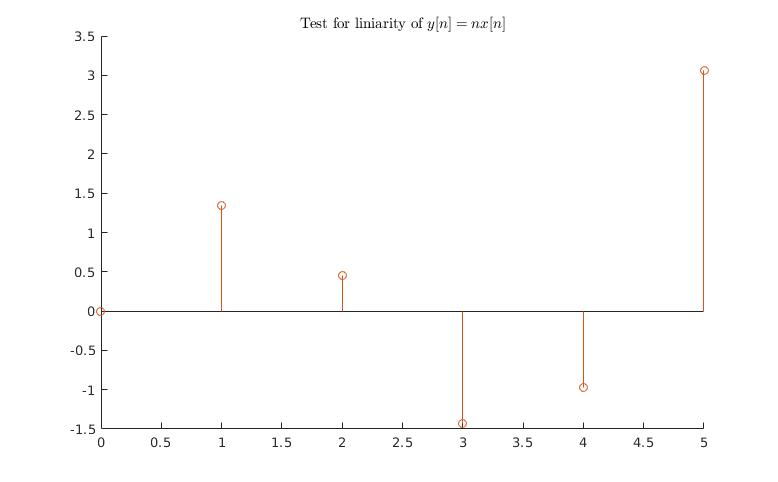
\includegraphics[width=10cm]{linarity_test_2.jpg}
\caption{$f(x_1+x_2) = f(x_1)+f(x_2)$}
\end{figure}
\newpage

\section*{Convolution}
The functions $h[n]=0.7^n$ and $x[n]=u[n]-u[n-4]$ were convolved in matlab, and by hand, to produce the function $y[n]$.\\
\begin{figure}[h]
\centering
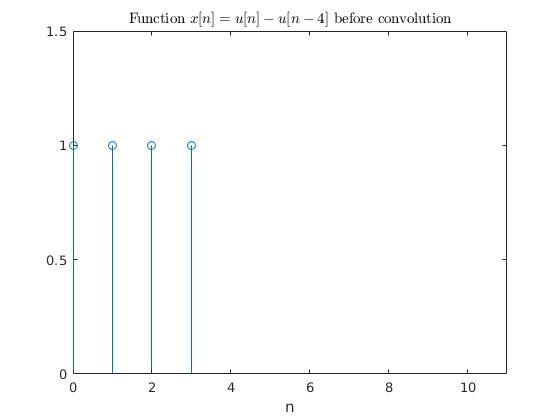
\includegraphics[width=11cm]{x(n).jpg}
\caption{$h[n]=0.7^n$}
\end{figure}
\begin{figure}[h]
\centering
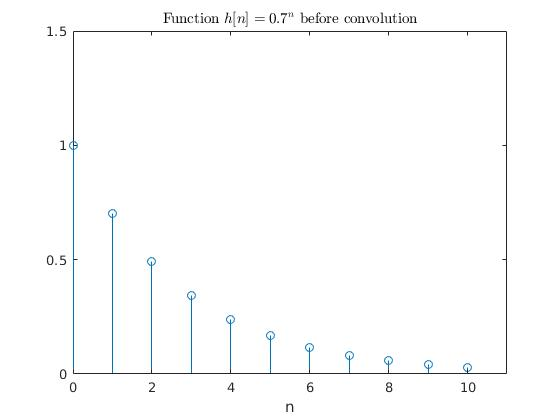
\includegraphics[width=11cm]{h(n).jpg}
\caption{$x[n]=u[n]-u[n-4]$}
\end{figure}
\newpage

The output of this convolution done in matlab can be seen in figure 6.\\
\begin{figure}[h]
\centering
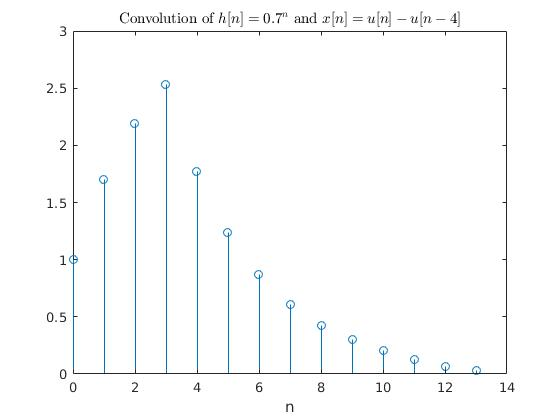
\includegraphics[width=11cm]{Convolution.jpg}
\caption{Convolution of $x[n]$ with $h[n]$}
\end{figure}

The output of the convolution done by hand can be seen to be exactly the same in figure 7, with the working below in figure 8.\\

\begin{figure}[h]
\centering
\includegraphics[width=11cm]{Convolutionbyhand.jpg}
\caption{Convolution of $x[n]$ with $h[n]$ bone by hand}
\end{figure}


\begin{figure}[h]
\centering
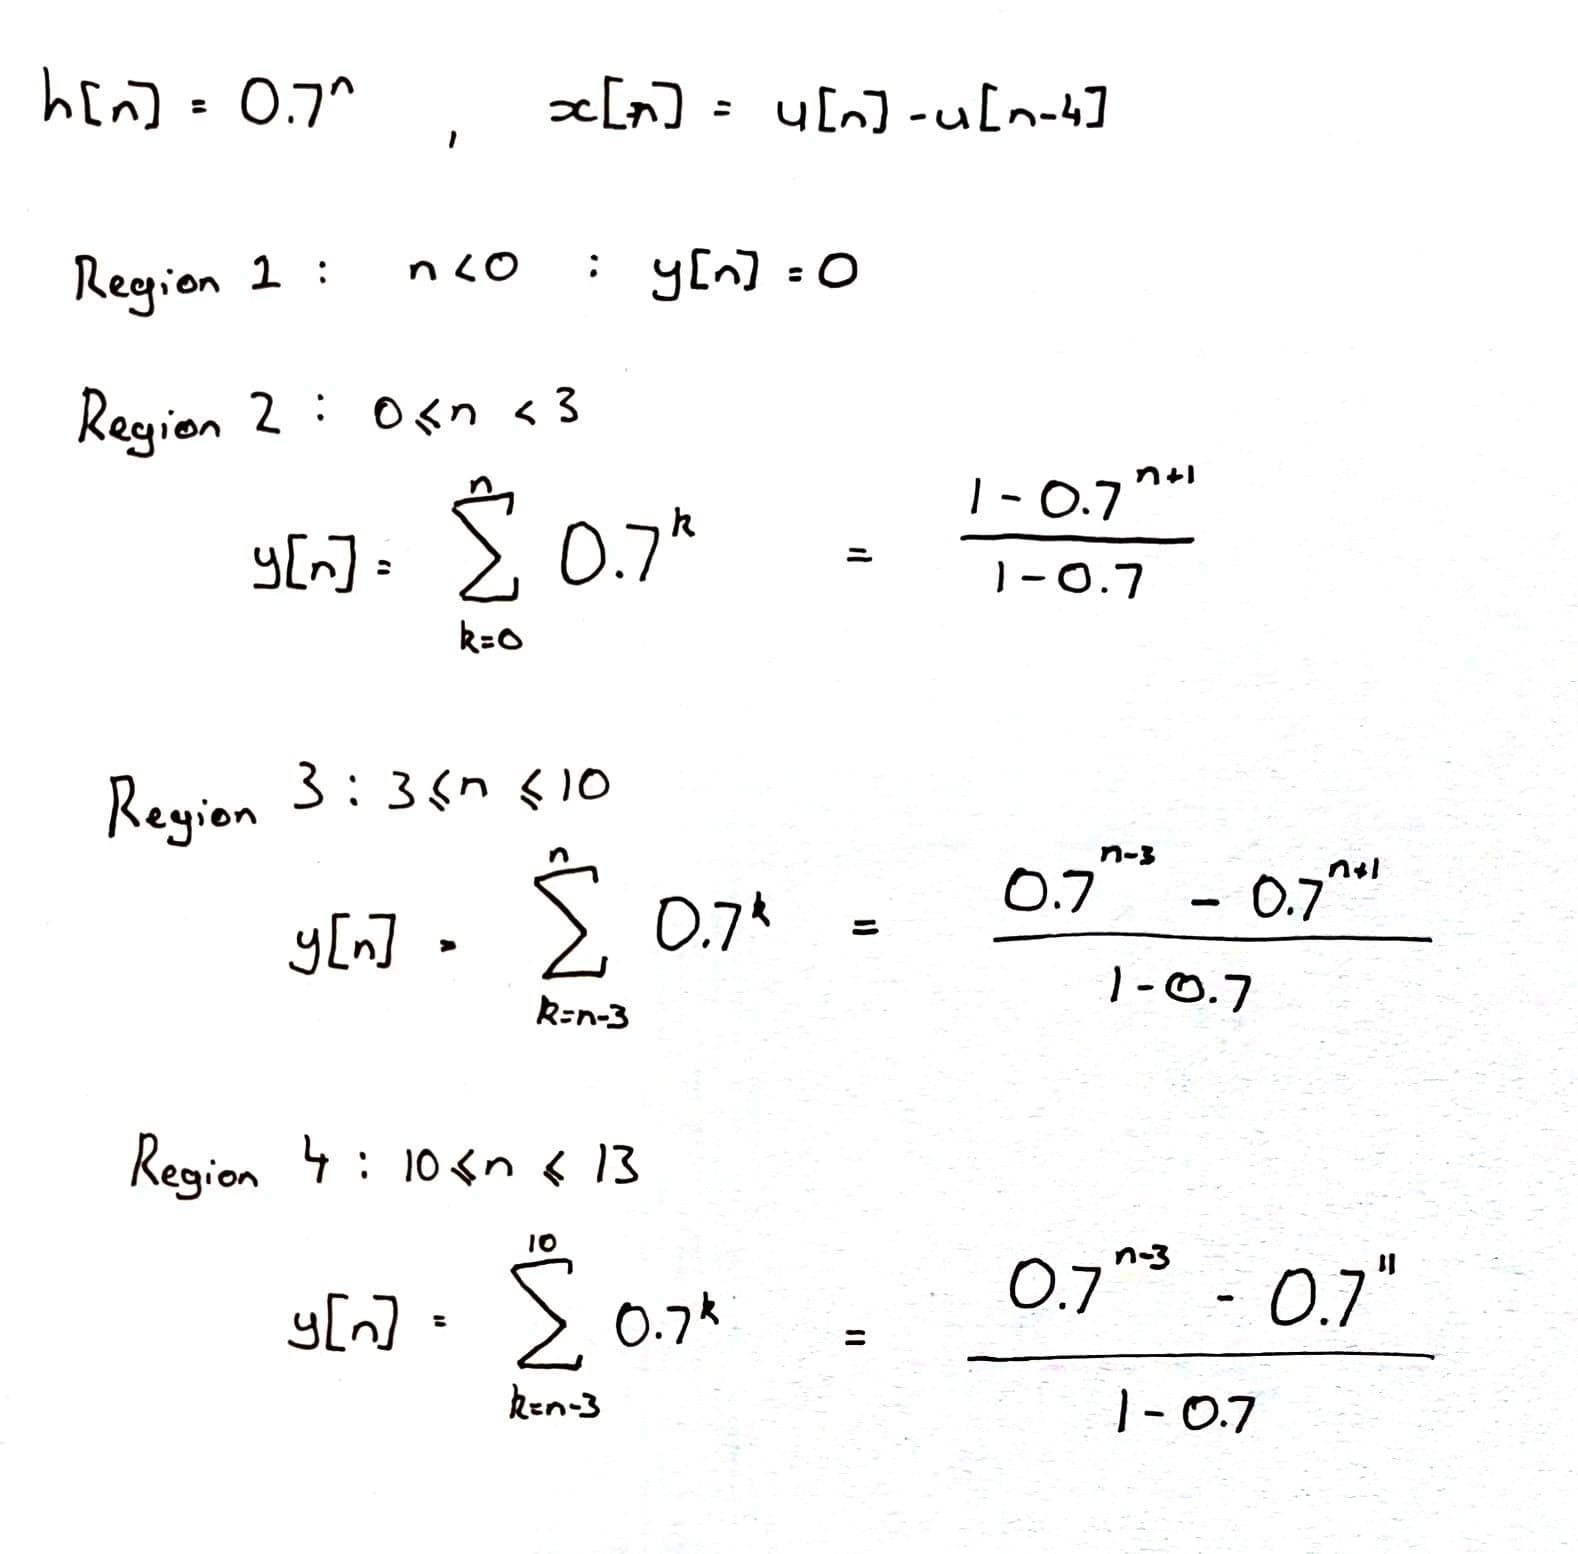
\includegraphics[width=\linewidth]{conv.jpg}
\caption{Convolution of $x[n]$ with $h[n]$ working}
\end{figure}
\newpage

\lstset{language=Matlab,%
    %basicstyle=\color{red},
    breaklines=true,%
    morekeywords={matlab2tikz},
    keywordstyle=\color{blue},%
    morekeywords=[2]{1}, keywordstyle=[2]{\color{black}},
    identifierstyle=\color{black},%
    stringstyle=\color{mylilas},
    commentstyle=\color{mygreen},%
    showstringspaces=false,%without this there will be a symbol in the places where there is a space
    numbers=left,%
    numberstyle={\tiny \color{black}},% size of the numbers
    numbersep=9pt, % this defines how far the numbers are from the text
    emph=[1]{for,end,break},emphstyle=[1]\color{red}, %some words to emphasise
    %emph=[2]{word1,word2}, emphstyle=[2]{style},    
}


\section*{Matlab Code}

\lstinputlisting{lab_1.m}

\end{document}
